\documentclass[aspectratio=1610, 10pt, notheorems]{beamer}
\usetheme{Berkeley}
\usecolortheme{seahorse}

%%% Кодировка и локализация %%%
\usepackage[utf8]{inputenc} % кодовая страница документа
\usepackage[T2A]{fontenc} % внутренняя кодировка  TeX
\usepackage[english,russian]{babel} % локализация и переносы

%%% Гипперссылки и pdf %%%
\usepackage{cmap} % русский поиск в pdf
\usepackage{hyperref} % гиперссылки

%%% Пакеты для формул %%%
\usepackage{amsmath} % удобная вёрстка многострочных формул, масштабирующийся текст в формулах, формулы в рамках и др.
\usepackage{amssymb} % несколько сотен дополнительных математических символов
\usepackage{amsthm} % окружения «теорема», «лемма» и т. п.
\usepackage{amsfonts} % Ажурный \mathbb{} и готический \mathfrak{} шрифты
\usepackage{mathrsfs} % Mathematical Script letters (шрифт Эйлера) \mathscr{}
\usepackage{euscript} % Шрифт Евклида \EuScript{}
% каллиграфический шрифт \mathcal{} не требует пакета
%\usepackage{enumitem}
\usepackage{bm}
\usepackage{multicol}

%%% Графика, изображения и цвета %%%
\usepackage{graphicx} % Работа с графикой \includegraphics{}
\usepackage{float} % Фиксация плавабщих боксов [H]
\graphicspath{
    {./images/}, 
    {./images/img1/}, 
    {./images/img2/}, 
    {./images/img3/}, 
    {./images/tikz1/}, 
    {./images/tikz2/}, 
    {./images/tikz3/},
    {./images/tree/},
    {./images/presentation/},
    }
    
\newtheorem{theorem}     {Теорема}
\newtheorem{lemma}       {Лемма}
\newtheorem{proposition} {Предложение}
\newtheorem{corollary}   {Следствие}
\newtheorem{definition}  {Определение}
\newtheorem{example}     {Пример} 
\newtheorem{remark}      {Замечание}
   
%%% Настройки презентации %%%
\everymath{\color{blue}}    % цвет формул в текстмоде
\everydisplay{\color{blue}} % цвет выключных формул
\setbeamertemplate{navigation symbols}{} % Убрать панель навигации
% \setbeamertemplate{footline}[frame number] % Номера слайдов вместо нижней строки
%\setbeamertemplate{page number in head/foot}[totalframenumber]
%\setbeamertemplate{bibliography item}{\insertbiblabel}
\hypersetup{unicode=true} % разрешить использование символов Юникод в закладках. настройка для hiperref
\logo{
\includegraphics[width=1.4cm]{LogoIM.png}}

%%% Русская традиция начертания математических знаков
\renewcommand{\le}  {\ensuremath{\leqslant}}
\renewcommand{\leq} {\ensuremath{\leqslant}}
\renewcommand{\ge}  {\ensuremath{\geqslant}}
\renewcommand{\geq} {\ensuremath{\geqslant}}
\renewcommand{\emptyset}{\varnothing}

%%% Русская традиция начертания математических функций (на случай копирования из зарубежных источников)
\renewcommand{\tan}{\operatorname{tg}}
\renewcommand{\cot}{\operatorname{ctg}}
\renewcommand{\csc}{\operatorname{cosec}}

%%% Русская традиция начертания греческих букв (греческие буквы вертикальные, через пакет upgreek)
% \usepackage{upgreek} % прямые греческие ради русской традиции
% \renewcommand{\epsilon}{\ensuremath{\upvarepsilon}}   %  русская традиция записи
% \renewcommand{\phi}{\ensuremath{\upvarphi}}
% %\renewcommand{\kappa}{\ensuremath{\varkappa}}
% \renewcommand{\alpha}{\upalpha}
% \renewcommand{\beta}{\upbeta}
% \renewcommand{\gamma}{\upgamma}
% \renewcommand{\delta}{\updelta}
% \renewcommand{\varepsilon}{\upvarepsilon}
% \renewcommand{\zeta}{\upzeta}
% \renewcommand{\eta}{\upeta}
% \renewcommand{\theta}{\uptheta}
% \renewcommand{\vartheta}{\upvartheta}
% \renewcommand{\iota}{\upiota}
% \renewcommand{\kappa}{\upkappa}
% \renewcommand{\lambda}{\uplambda}
% \renewcommand{\mu}{\upmu}
% \renewcommand{\nu}{\upnu}
% \renewcommand{\xi}{\upxi}
% \renewcommand{\pi}{\uppi}
% \renewcommand{\varpi}{\upvarpi}
% \renewcommand{\rho}{\uprho}
% %\renewcommand{\varrho}{\upvarrho}
% \renewcommand{\sigma}{\upsigma}
% %\renewcommand{\varsigma}{\upvarsigma}
% \renewcommand{\tau}{\uptau}
% \renewcommand{\upsilon}{\upupsilon}
% \renewcommand{\varphi}{\upvarphi}
% \renewcommand{\chi}{\upchi}
% \renewcommand{\psi}{\uppsi}
% \renewcommand{\omega}{\upomega}



\newcommand {\rr}  {\mathbb{R}}
\newcommand {\nn}  {\mathbb{N}}
\newcommand {\zz}  {\mathbb{Z}}
\newcommand {\bbc} {\mathbb{C}}
% \newcommand {\rd}  {\mathbb{R}^d}
% \newcommand {\rpo} {\mathbb{R}_+^1}

\newcommand {\al} {\alpha}
\newcommand {\be} {\beta}
\newcommand {\da} {\delta}
\newcommand {\Da} {\Delta}
\newcommand {\Dl} {\Delta}
\newcommand {\ga} {\gamma}
\newcommand {\Ga} {\Gamma}
\newcommand {\la} {\lambda}
\newcommand {\La} {\Lambda}
\newcommand {\om} {\omega}
\newcommand {\Om} {\Omega}
\newcommand {\sa} {\sigma}
\newcommand {\Sa} {\Sigma}
\newcommand {\te} {\theta}
\newcommand {\fy} {\varphi}
\newcommand {\Fy} {\varPhi}
\newcommand {\ep} {\varepsilon}
\newcommand {\ro} {\varrho}

\newcommand{\bd}{{\bm{d}}}
\newcommand{\bj}{{\bm{j}}}
\newcommand{\bi}{{\bm{i}}}
\newcommand{\bk}{{\bm{k}}}
\newcommand{\bu}{{\bm{u}}}
\newcommand{\bx}{{\bm{x}}}
\newcommand{\bl}{{\bf{l}}}
\newcommand{\bma}{{\bm{\alpha}}}
\newcommand{\bmb}{{\bm{\beta}}}
\newcommand{\bmg}{{\bm{\gamma}}}

\newcommand {\ra}  {\rightarrow}
\newcommand {\IN}  {\subset}
\newcommand {\NI}  {\supset}
\newcommand {\mmm} {\setminus}
\newcommand {\8}   {\infty}
\newcommand {\io}  {I^\infty}
\newcommand {\ia}  {I^*}
\newcommand {\0}   {\varnothing}
\newcommand {\dd}  {\partial}
\newcommand {\pr}  {\mathrm{pr}}
% \renewcommand{\span}{\mathrm{span}}


\newcommand {\eA} {{\EuScript A}}
\newcommand {\eJ} {{\EuScript J}}
\newcommand {\eC} {{\EuScript C}}
\newcommand {\eU} {{\EuScript U}}
\newcommand {\eP} {{\EuScript P}}
\newcommand {\eS} {{\EuScript S}}
\newcommand {\eW} {{\EuScript W}}
\newcommand {\eZ} {{\EuScript Z}}
\newcommand {\eK} {{\EuScript K}}
\newcommand {\hT} {{\hat T}}
\newcommand {\wP} {{\widetilde P}}
\newcommand {\eV} {{\mathcal V}}

\def \diam {\mathop{\rm diam} \nolimits}
\def \sup  {\mathop{\rm sup}  \nolimits}
\def \fix  {\mathop{\rm fix}  \nolimits}
\def \Lip  {\mathop{\rm Lip}  \nolimits}
\def \min  {\mathop{\rm min}  \nolimits}
\def \Ln   {\mathop{\rm Ln}   \nolimits}
\def \Id   {\mathop{\rm Id}   \nolimits}

\newcommand{\red}{\textcolor{red}}     % Новые переменные и переименования

%%% Данные для титульного листа %%%
\title[ ]
    {Анализ на самоподобных множествах с конечным пересечением}
\author[ ]
    {Дроздов Дмитрий Алексеевич\\ \; \\
    Научный руководитель:\\ 
    д. ф.-м. н., доцент Тетенов Андрей Викторович}
\institute[ИМ СО РАН]{Институт математики имени С. Л. Соболева СО РАН}
\date[10.06.2024]
    {Защита диссертации на соискание ученой степени\\ кандидата физико-математических наук по специальности \\1.1.1 Вещественный, комплексный и функциональный анализ\\ \; \\
    16.12.2024}


\begin{document}


\begin{frame}{}
    \titlepage
\end{frame}

%\begin{frame}{}
%\tableofcontents
%\end{frame}

\section{Выносимые на защиту положения} 

\begin{frame}{Выносимые на защиту положения}

{\normalsize
\begin{enumerate}
\item Найдено необходимое условие, при котором аттрактор обобщённой полигональной системы является дендритом.
\item Доказано, что при достаточно малом $\delta=\delta(\eS)>0$ аттрактор любой (удовлетворяющей условию совпадения параметров) $\delta$-деформации $\eS'$ полигональной системы $\eS$ является дендритом, изоморфным аттрактору системы $\eS$.
\item Получена формула, выражающая пересечение двух фрактальных $k$-кубов в терминах их множеств единиц.
Найдены условия, при которых такое пересечение будет пустым, конечным, счётным и несчётным.
Для конечного пересечения получена оценка мощности.
\item Разработан алгоритм, позволяющий проверить, является ли фрактальный $k$-куб дендритом с одноточечным пересечением.
\item Доказано, что нетривиальные односвязные фрактальные квадраты являются дендритами со свойством одноточечного пересечения.
\item Доказано, что нетривиальные односвязные фрактальные квадраты допускают ровно семь возможных топологических типов главного дерева.
\end{enumerate}}
\end{frame}


\section{Вводные понятия} %


\begin{frame}{Вводные понятия}{Самоподобное множество}
    \begin{definition}[Hutchinson J. E. (1981)]
        Пусть $\eS=\{S_1, \ldots, S_m\}$ --- система сжимающих подобий в $\mathbb{R}^n$.  
        Непустой компакт $K$, удовлетворяющий уравнению  $K=\bigcup\limits_{i=1}^m S_i(K)$, будем называть {\em аттрактором системы} $\eS$ или множеством, самоподобным (инвариантным) относительно системы $\eS$.
    \end{definition}
%    \begin{block}{}
%        Для системы $\eS=\{S_1,\ldots,S_m\}$ сжимающих подобий в $\rr^n$  равенством $T(A)=\bigcup\limits_{i=1}^m S_i(A)$ задаётся  оператор Хатчинсона на $C(\rr^n)$.
%    \end{block}
    % Мы обозначим как $I=\{1, \ldots, m\}$ множество индексов системы $\eS$, а также обозначим как $I^{*}=\bigcup\limits_{n=1}^\infty I^n$ множество слов $\bm{i}=i_1\ldots i_n$ конечной длинны алфавита $I$, называемых {\em мультииндексами}.
    % Мы будем использовать сокращение $S_{\bj} = S_{j_{1}j_{2}\ldots j_{n}}=S_{j_{1}}S_{j_{2}} \ldots S_{j_{n}}$ и обозначим $S_{\bj}(K)$ как $K_{\bj}$.
    % Множество $K_\bj$,  где $\bj=j_{1}j_{2}\ldots j_{n}$,  будем называть {\em копией порядка (итерации) $n$} множества $K$.
    \begin{center}
    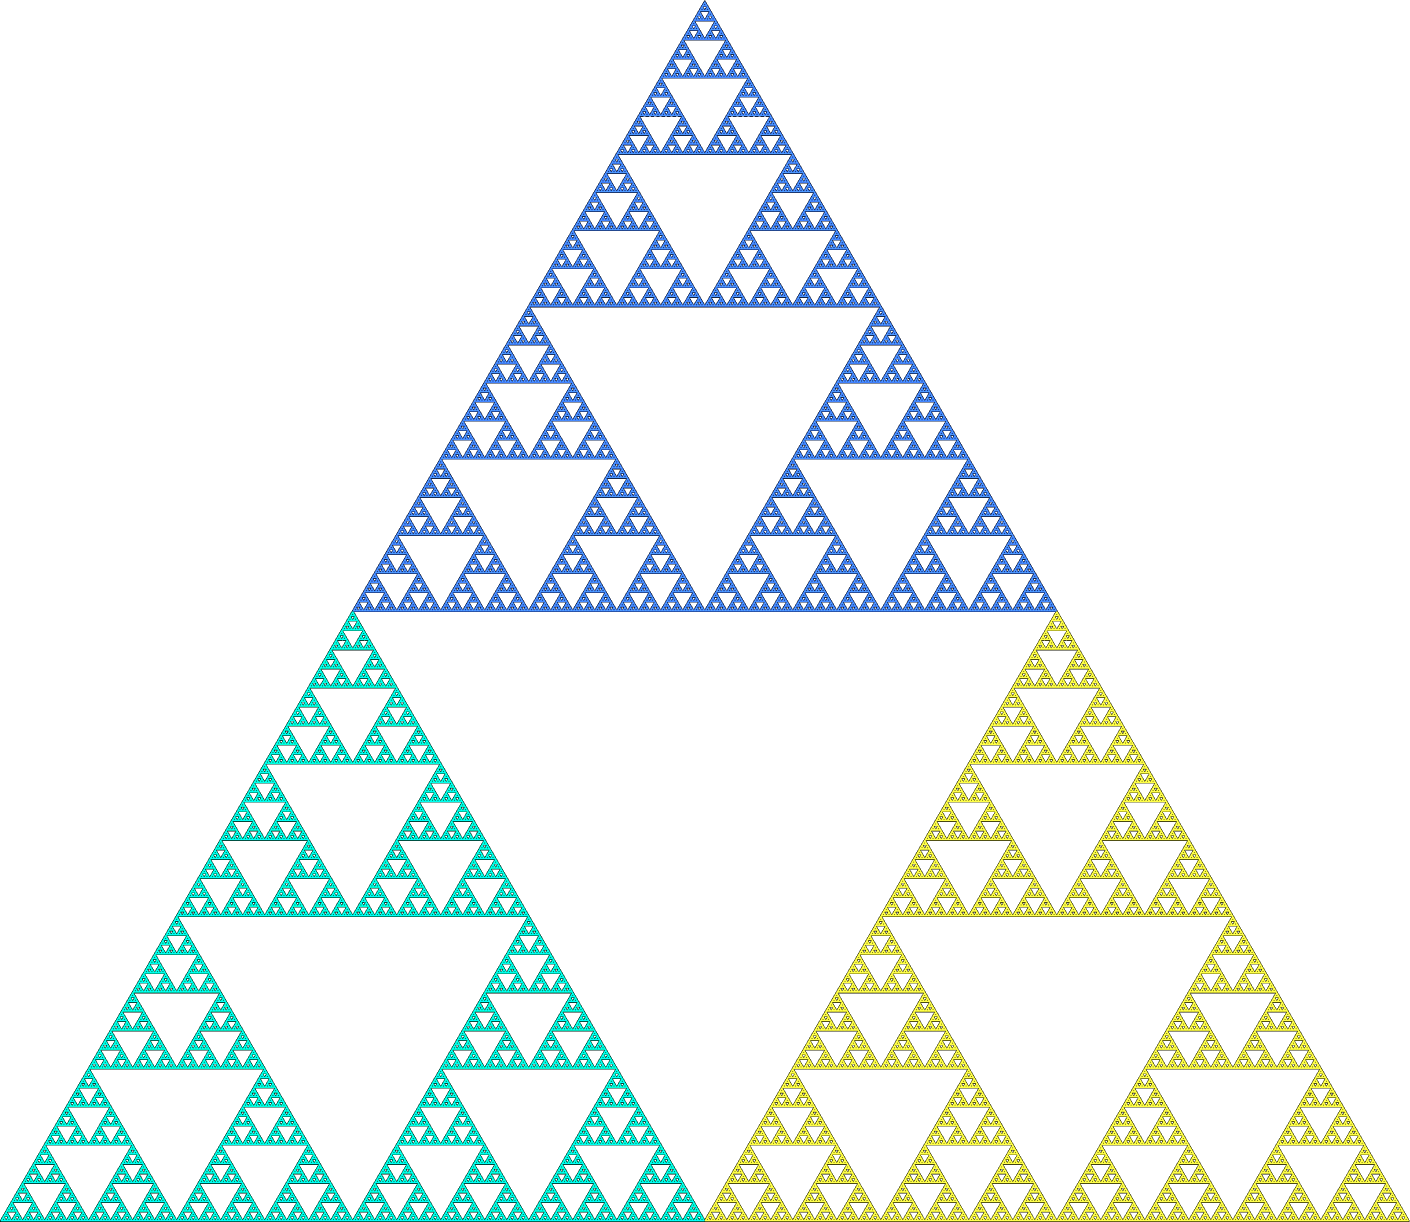
\includegraphics[width=0.4\textwidth]{SerpTri.png}
    \end{center}
    \footnotetext[1]{Hutchinson J. E., Fractals and self-similarity, Indiana Univ. Math. J. \textbf{30} (1981), 713--747.}
\end{frame}


\begin{frame}{Вводные понятия}{Самоподобная граница}
%\begin{definition}
%{\em Самоподобной границей} аттрактора $K$ называется множество $\dd K$ всех $x\in K$ таких, по образам которых пересекаются друг с другом копии аттрактора $K$.
%\end{definition}
%Самоподобной границей аттрактора $K$ называется множество $\dd K$ всех $x\in K$ таких, по образам которых пересекаются друг с другом копии аттрактора $K$
\begin{definition}
% {\em Самоподобной границей} аттрактора $K$ называется множество $\dd K$ всех $x\in K$ таких, по образам которых пересекаются друг с другом копии аттрактора $K$.
Пусть $\eC:=\{x:\; x\in S_i(K)\cap S_j(K),\; i,j \in I, i\neq j\}$ ---  объединение всех попарных пересечений $S_i(K)\cap S_j(K)$ (при $i\neq j$) копий первой степени самоподобного множества $K$.
% Назовём такое $\eC$ {\em критическим множеством}.
% Каждая точка критического множества имеет как минимум два адреса в индексном пространстве.

Множество $\dd K:=\{x\in K: \text{существует }\bj\in I^* \text{ такое что } S_\bj(x)\in \eC\}$ назовём {\em самоподобной границей} для $K$.
\end{definition}
%Говоря иначе, самоподобная граница $\dd K$ --- это множество всех предшественников для точек из $\eC$.
\end{frame}


\begin{frame}{Вводные понятия}{Дендрит и его главное дерево}
\begin{columns}
\column{0.6\textwidth}
\begin{definition} 
Дендритом называется локально связный континуум, не содержащий простых замкнутых дуг.
\end{definition}
\;\par\;\par
\begin{definition}
Пусть $K$ --- самоподобный дендрит c конечной самоподобной границей $\dd K$. 
Минимальный поддендрит $\hat\gamma\IN K$, содержащий $\dd K$, называется {\em главным деревом} дендрита $K$.
\end{definition}
\column{0.4\textwidth}
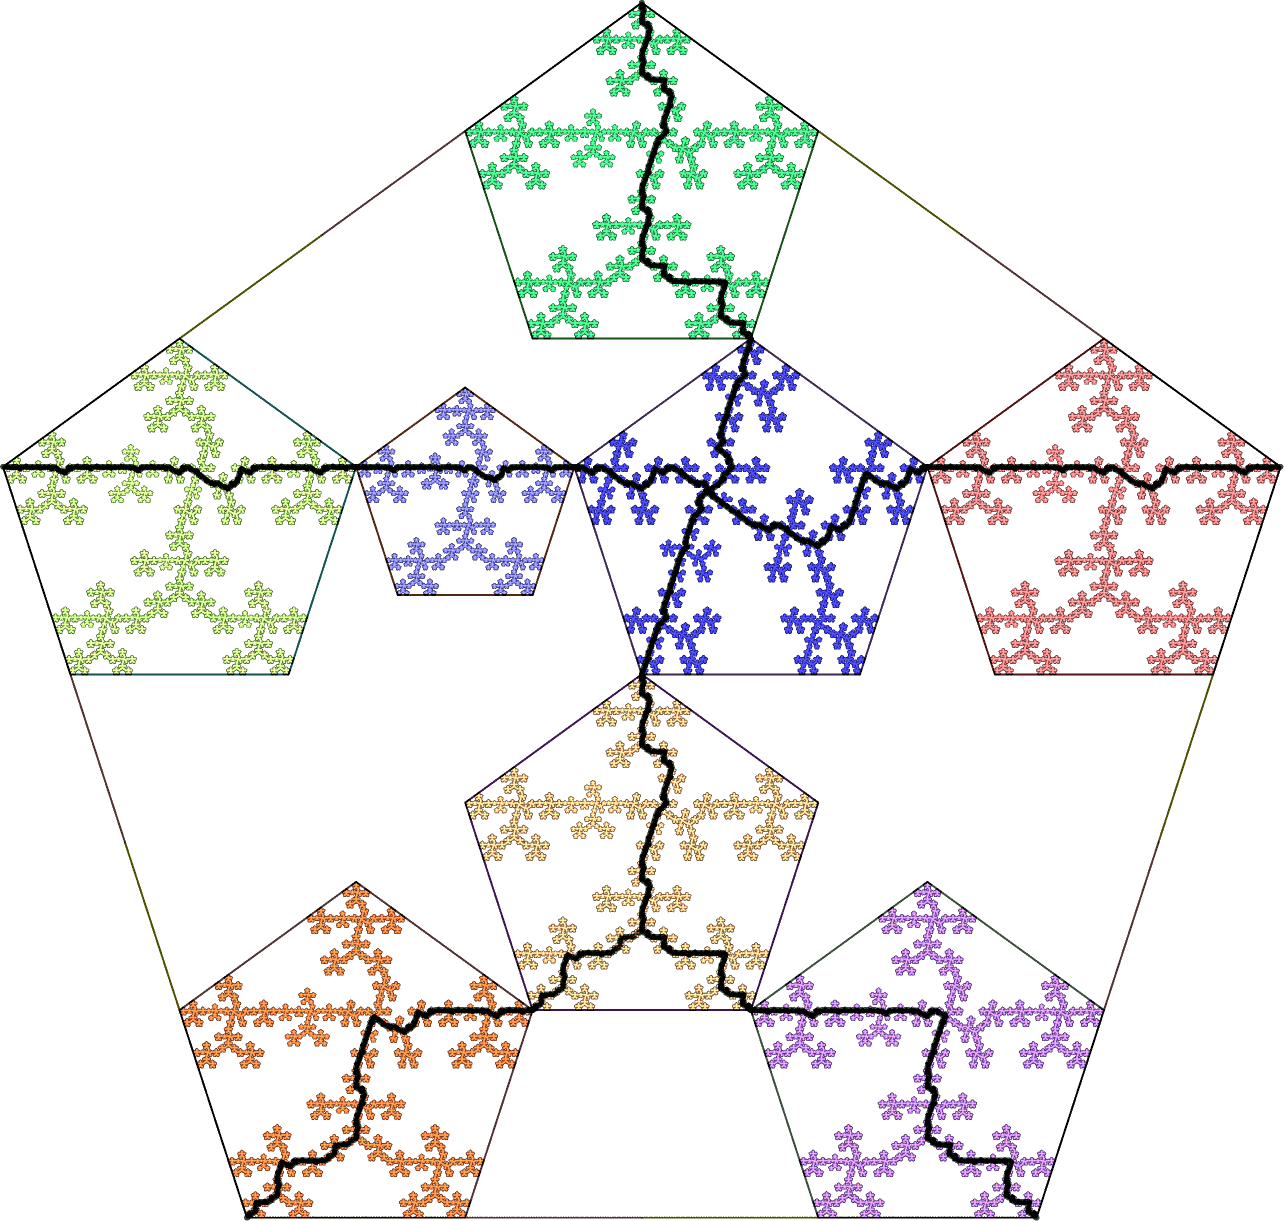
\includegraphics[width=\textwidth]{penta4plus3.png}
\end{columns}
%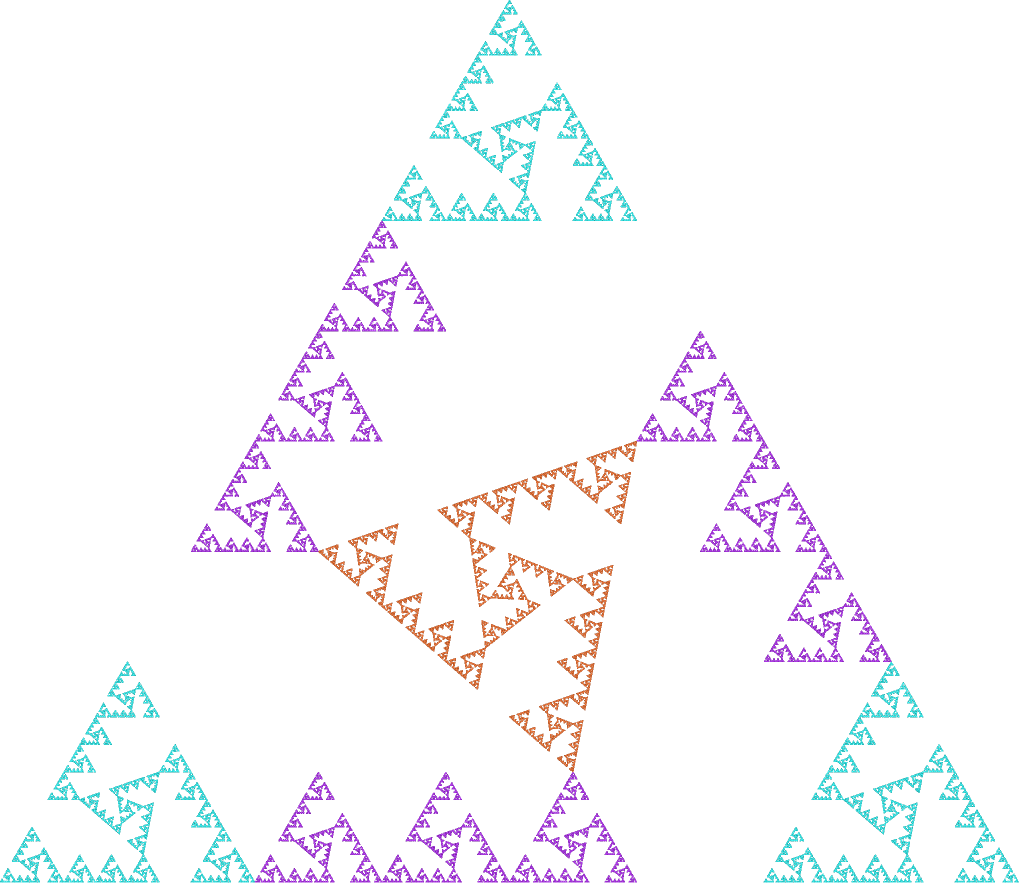
\includegraphics[width=0.48\textwidth]{tr_2f.png}
%\hfill
%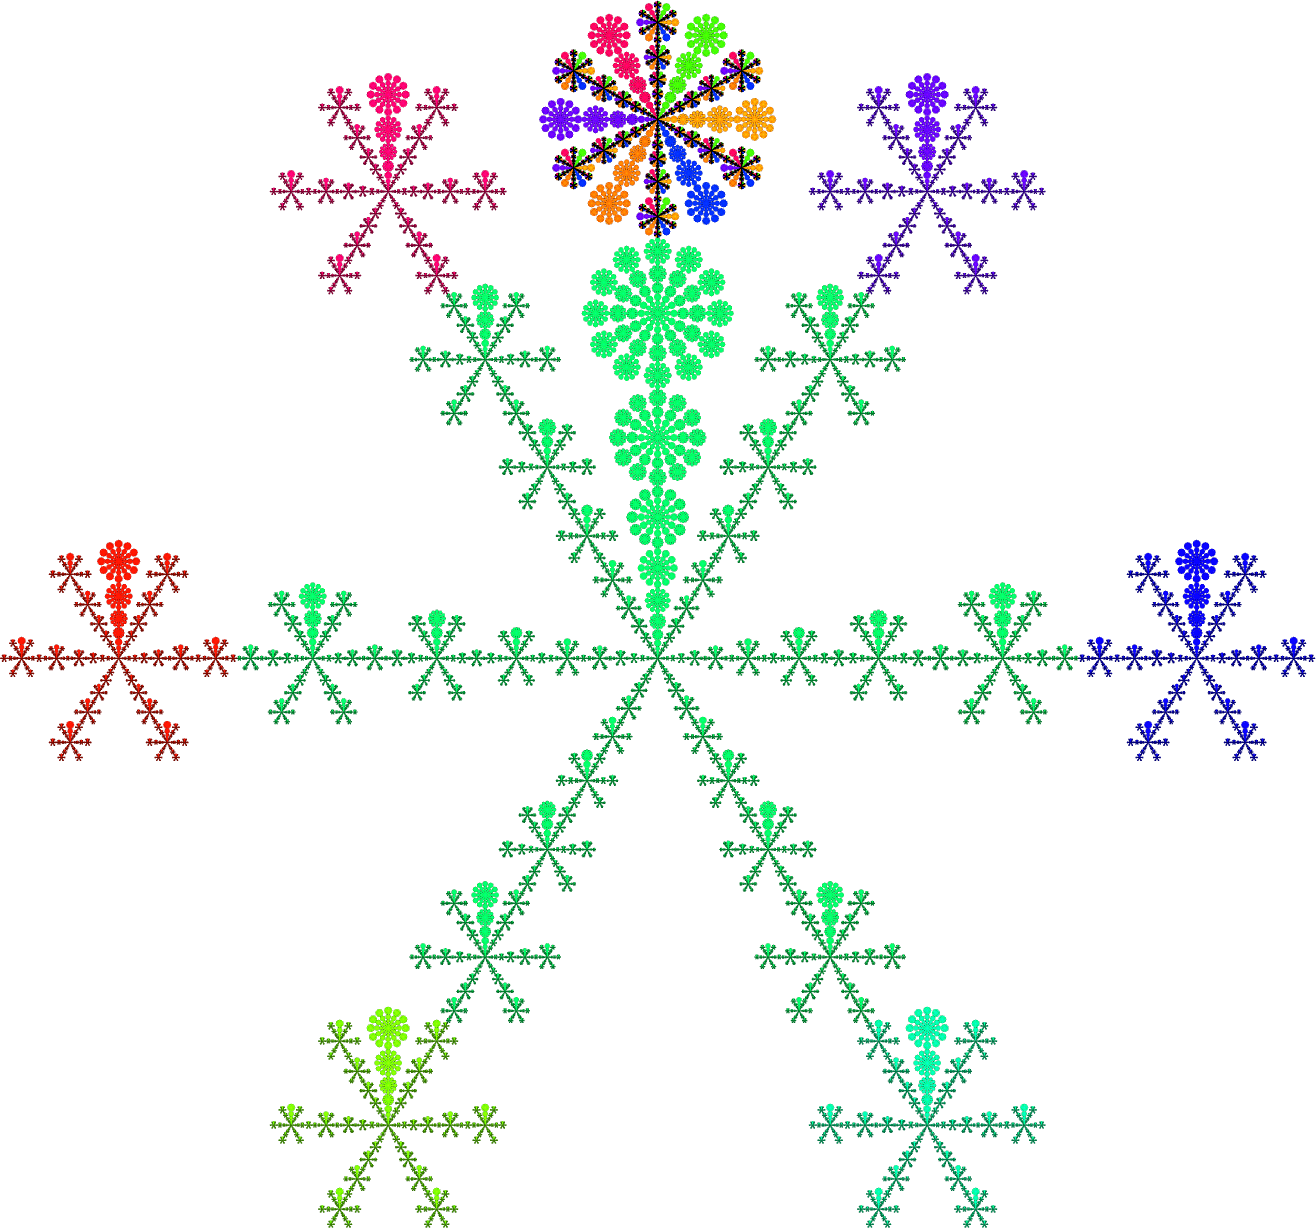
\includegraphics[width=0.45\textwidth]{den_int_6.png}

\end{frame}

\section{Деформации полигональных систем} %


\begin{frame}{Полигональные системы и их деформации}{История вопроса}
\begin{itemize}
    \item M. Hata (1985) --- критерий связности и некоторые свойства самоподобных дендритов;
    \item C. Bandt, K. Keller (1991) --- сформулировали достаточное условие того, что самоподобное множество есть дендрит;
    \item R. Strichartz (1999) --- полигаскеты и кратчайшие дуги;
    \item А. В. Тетенов, М. С. Самуэль, Д. А. Ваулин (2017) --- полигональные и полиэдральные системы, главное дерево;
    \item А. В. Тетенов (2021) --- доказал достаточное условие того, что самоподобное множество есть дендрит;
\end{itemize}
\end{frame}





\begin{frame}{Полигональные системы и их деформации}{Полигональные системы}
\only<1>{
Пусть $P\IN \mathbb R^2$ --- многоугольник, \\
$V_P=\{A_1,...,A_{n_P}\}$ --- множество его вершин, и\\
$\eS = \{S_1, \ldots, S_m\}$ -- система сжимающих подобий в $\mathbb R^2$ такая, что:\\
{\bf(D1)}  для любого $i\in I$, множество $P_i=S_i(P)\IN P$;\\
{\bf(D2)}  для любых $i\neq j,\ \   i, j \in I,$ $P_i \cap P_j=V_{P_i}\cap V_{P_j}$ ;\\
{\bf(D3)}  $V_P\IN \bigcup\limits_{i\in I}S_i(V_P)$;\\
{\bf(D4)}  множество    ${\wP} = \bigcup \limits_{i = 1}^m P_i$ односвязно.
\begin{definition}
Система \ $\eS $, удовлетворяющая условиям {\bf (D1)-(D4)},
называется полигональной системой подобий.
\end{definition}}
\only<2>{
\begin{theorem}[M. Samuel, A. V. Tetenov, D. A. Vaulin (2017)]
Аттрактор $K$  полигональной  системы подобий $\eS$ является дендритом.
\end{theorem}
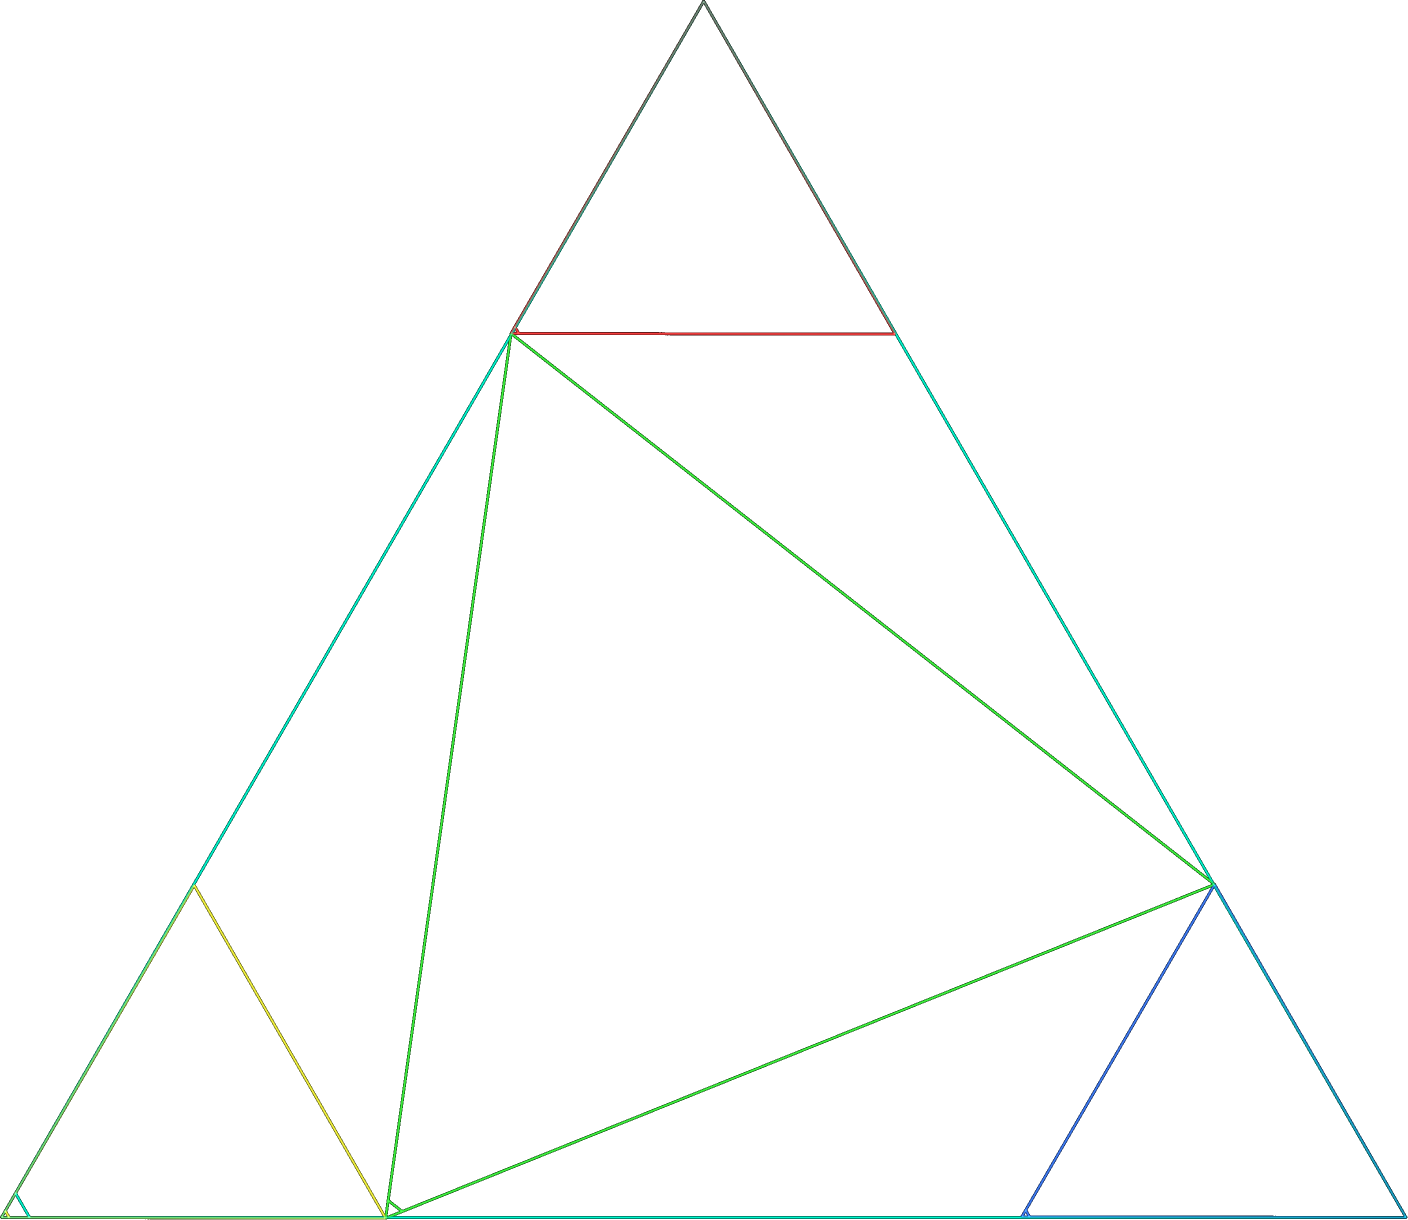
\includegraphics[width=0.45\textwidth]{CPS1_P.png}
\hfill
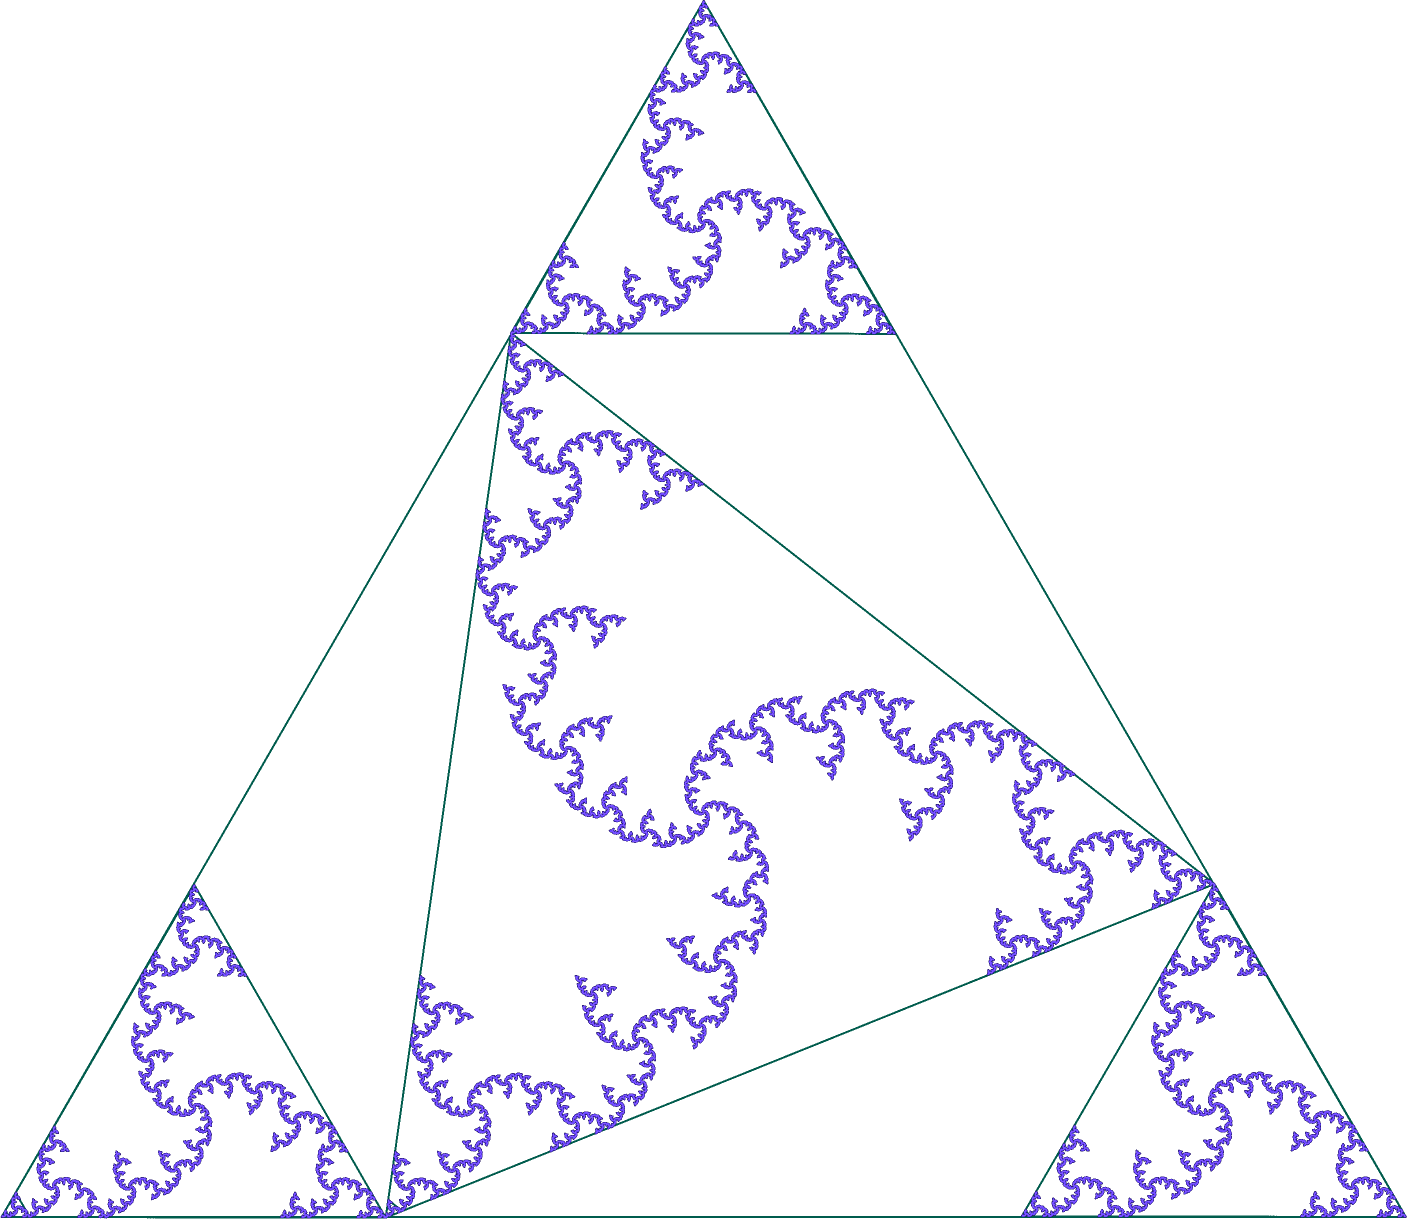
\includegraphics[width=0.45\textwidth]{CPS1_K.png}}
\end{frame}


\begin{frame}{Полигональные системы и их деформации}{Обобщённая полигональная система}
\begin{definition}	
Если опустить условие {\bf (D1)}, то система \ $\eS $, удовлетворяющая условиям {\bf (D2)-(D4)},
называется  обобщённой полигональной системой подобий.
\end{definition}
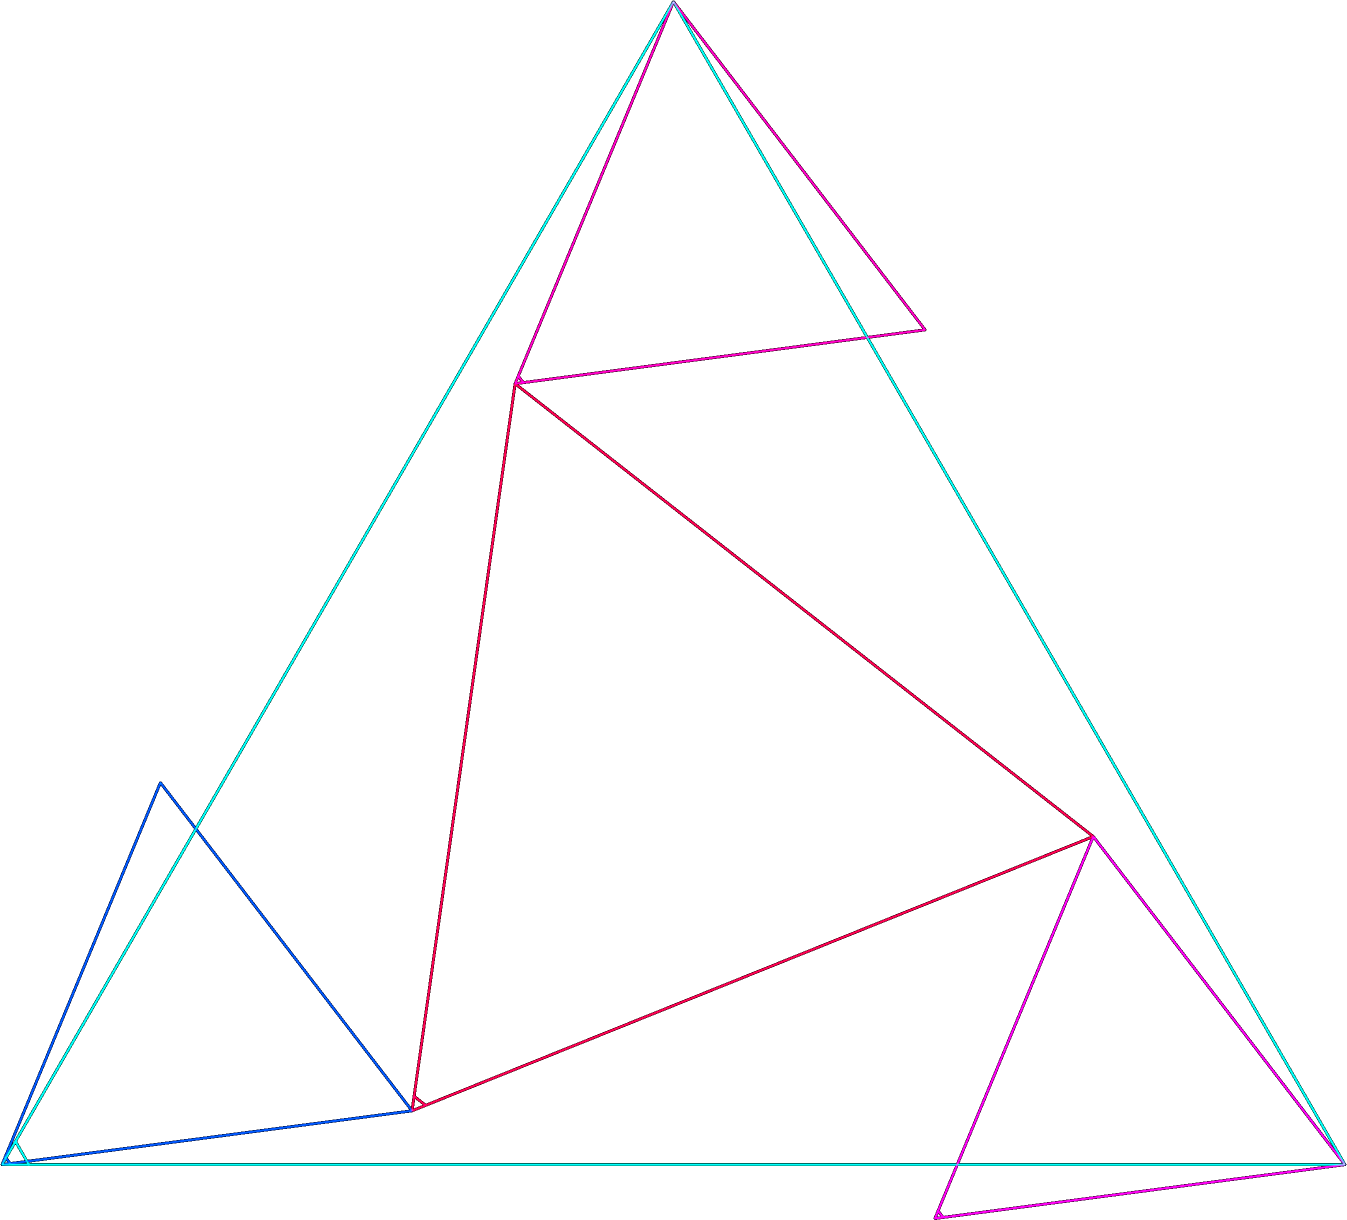
\includegraphics[width=0.45\textwidth]{def1_P.png}
\hfill
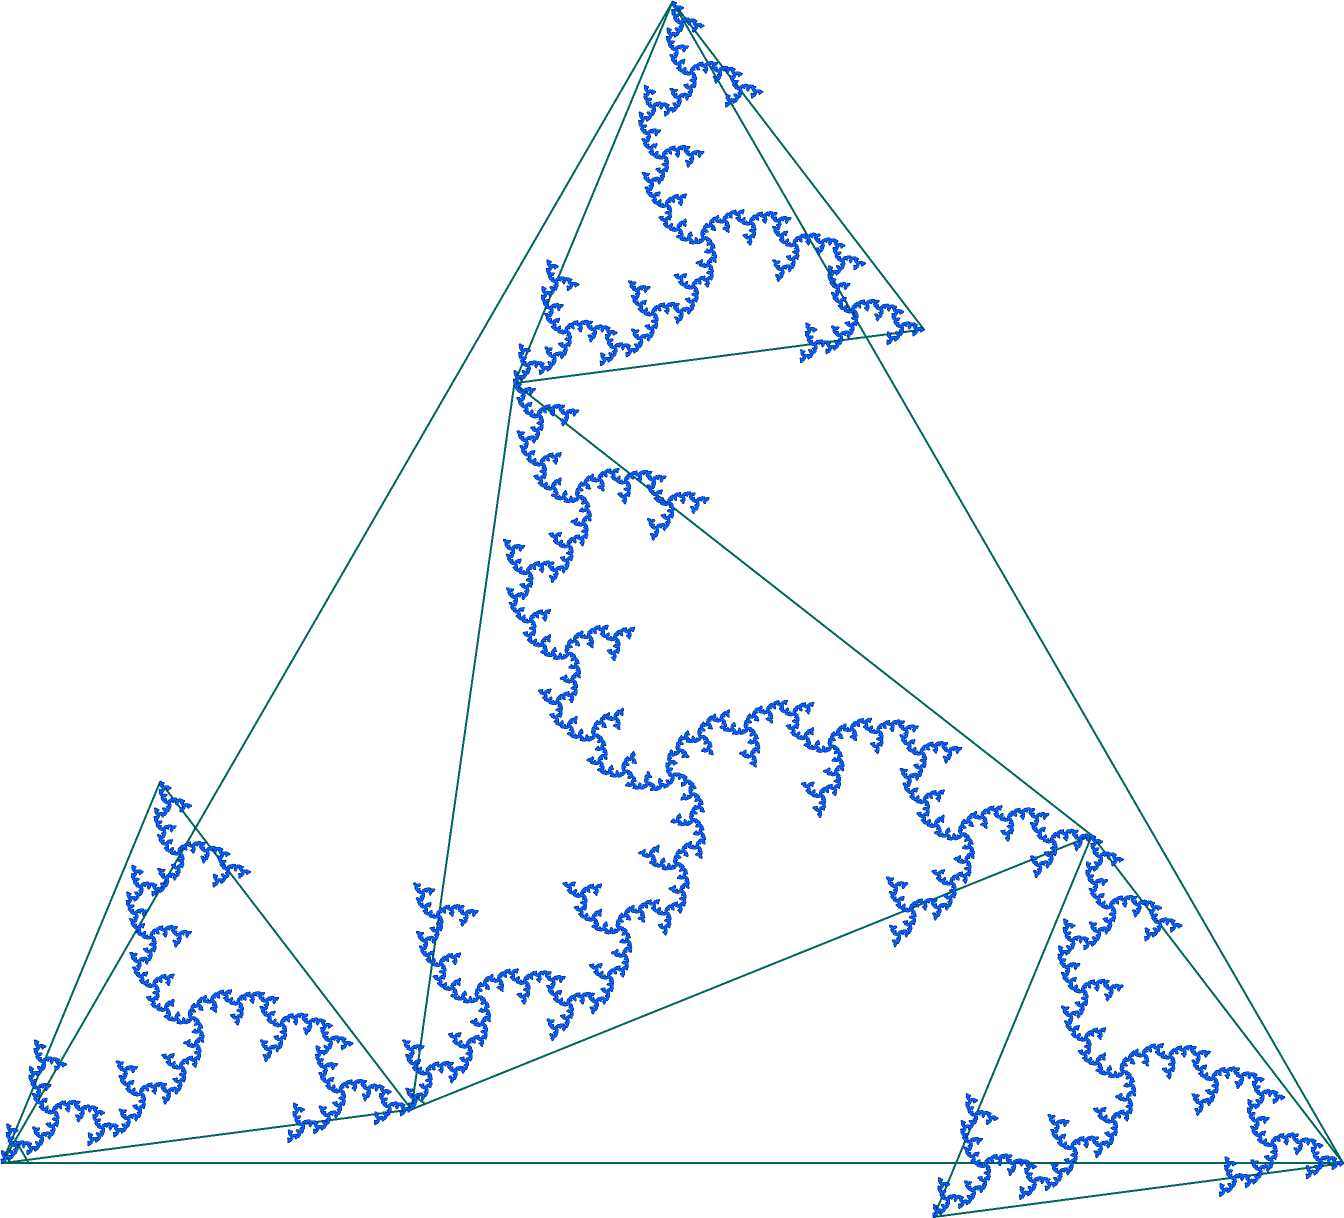
\includegraphics[width=0.45\textwidth]{def1_K.png}
\end{frame}


\begin{frame}{Полигональные системы и их деформации}{$\delta$-деформация}
\begin{definition}
Пусть $\delta>0$. 
Обобщенная $P'$-полигональная система $\eS'=\{S'_1,...,S'_m\}$ называется $\delta$-деформацией $P$-полигональной системы $\eS=\{S_1,...,S_m\}$, если существует биекция $f:\bigcup\limits_{k=1}^m V_{P_k}\to \bigcup\limits_{k=1}^m V_{P'_k}$ такая, что\\
a) $f|_{V_P}$ продолжается до гомеоморфизма $\tilde f: P\to  P'$; \\ 
b) $|f(x)-x|<\delta$  для любого $x\in \bigcup\limits_{k=1}^m V_{P_k}$\\  
c) $f(S_k(x))=S'_k(f(x))$ для любого $k\in I$ и $x\in V_P$.
\end{definition}
\end{frame}


%\begin{frame}{Инвариантная дуга и её параметр}
%\only<1>{
%Пусть $\eS=\{S_1,\ldots,S_m\}$ -- обобщённая $P$-полигональная система.
%$A_i$ -- общая вершина для $P$ и $S_i(P)$, причём $S_i(A_i)=A_i$.
%
%\begin{definition}
%Если дуга $\Gamma\IN K(\eS)$ такова, что $S_i(\Gamma)\IN\Gamma$, то мы говорим, что $\Gamma$ инвариантна относительно подобия $S_i$.
%\end{definition}
%
% \begin{definition}
%Пусть $\rho_i=\Lip(S_i)$ и $\alpha_i=\Delta\underset{\Gamma\mmm S_i(\Gamma)}{\arg}(z-A_i)$.
%Параметром дуги $\Gamma$ относительно $A_i$ называется отношение $\lambda_i=\dfrac{\alpha_i}{\ln\rho_i}.$    
% \end{definition}
%}

%\only<2>{
%\begin{center}
%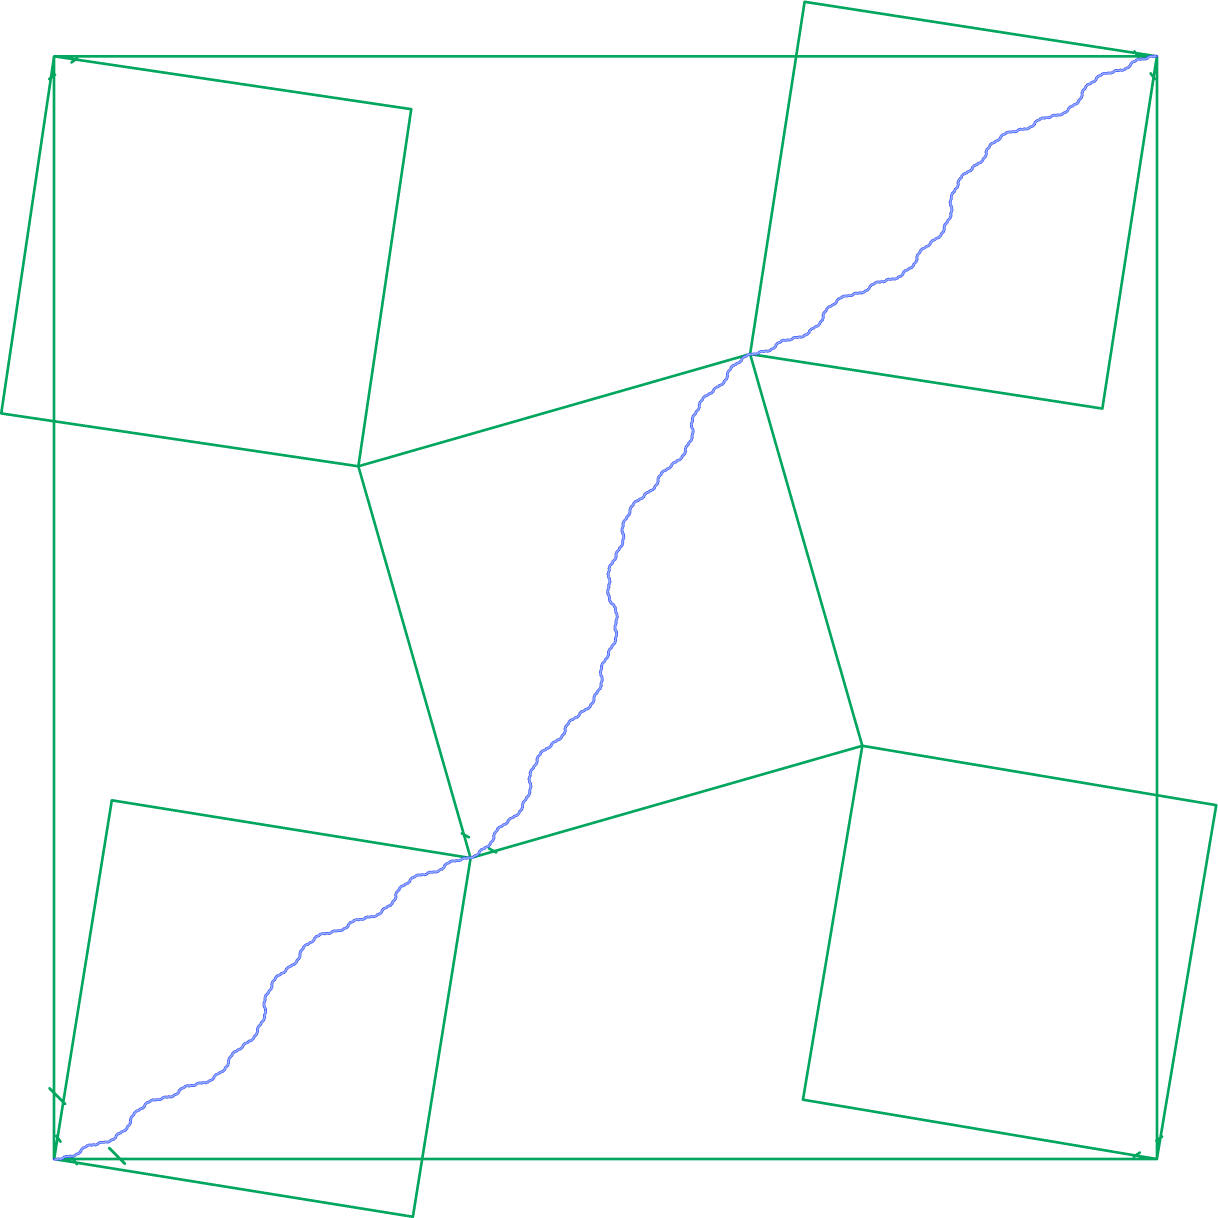
\includegraphics[width=0.6\textwidth]{InvArc1.png}
%\end{center}}
%\end{frame}

%\begin{frame}{Лемма о непересекающихся периодических дугах}
%\begin{lemma}[В. В. Асеев, А. В. Тетенов, А. С. Кравченко (2003)]
%Пусть $\Gamma_1$ и $\Gamma_2$ -- такие жордановы дуги с общим началом в $0$ и  концами $z_1$ и $z_2$ ($|z_1|=|z_2|=1$), что $\Gamma_1\cap\Gamma_2=\{0\}$.\\
%Если сжимающие подобия $S_1(z)=\rho_1 e^{i\alpha}z$ и $S_2(z)=\rho_2 e^{i\beta}z$ таковы, что $S_1(\Gamma_1)\IN\Gamma_1$ и $S_2(\Gamma_2)\IN\Gamma_2$,\\ 
%а $\alpha:=\Delta\underset{{\Gamma_1\mmm S_1(\Gamma_1)}}{\mathrm {Arg}}(z)$ и $\beta:=\Delta\underset{{\Gamma_2\mmm S_2(\Gamma_2)}}{\mathrm {Arg}}(z)$, то
%$$\lambda_1:=\dfrac{\alpha}{\ln\rho_1} = \lambda_2:=\dfrac{\beta}{\ln\rho_2}$$
%\end{lemma}
%
%\footnotetext[2]{В. В. Асеев, А. В. Тетенов, А. С. Кравченко, О самоподобных жордановых кривых на плоскости, Сиб. матем. журн., 44:3 (2003), 481–492}
%\end{frame}
%
%\begin{frame}{}
%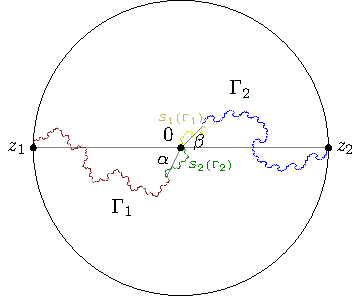
\includegraphics[width=0.8\textwidth]{2arc.pdf}
%\end{frame}

%\begin{frame}{}
%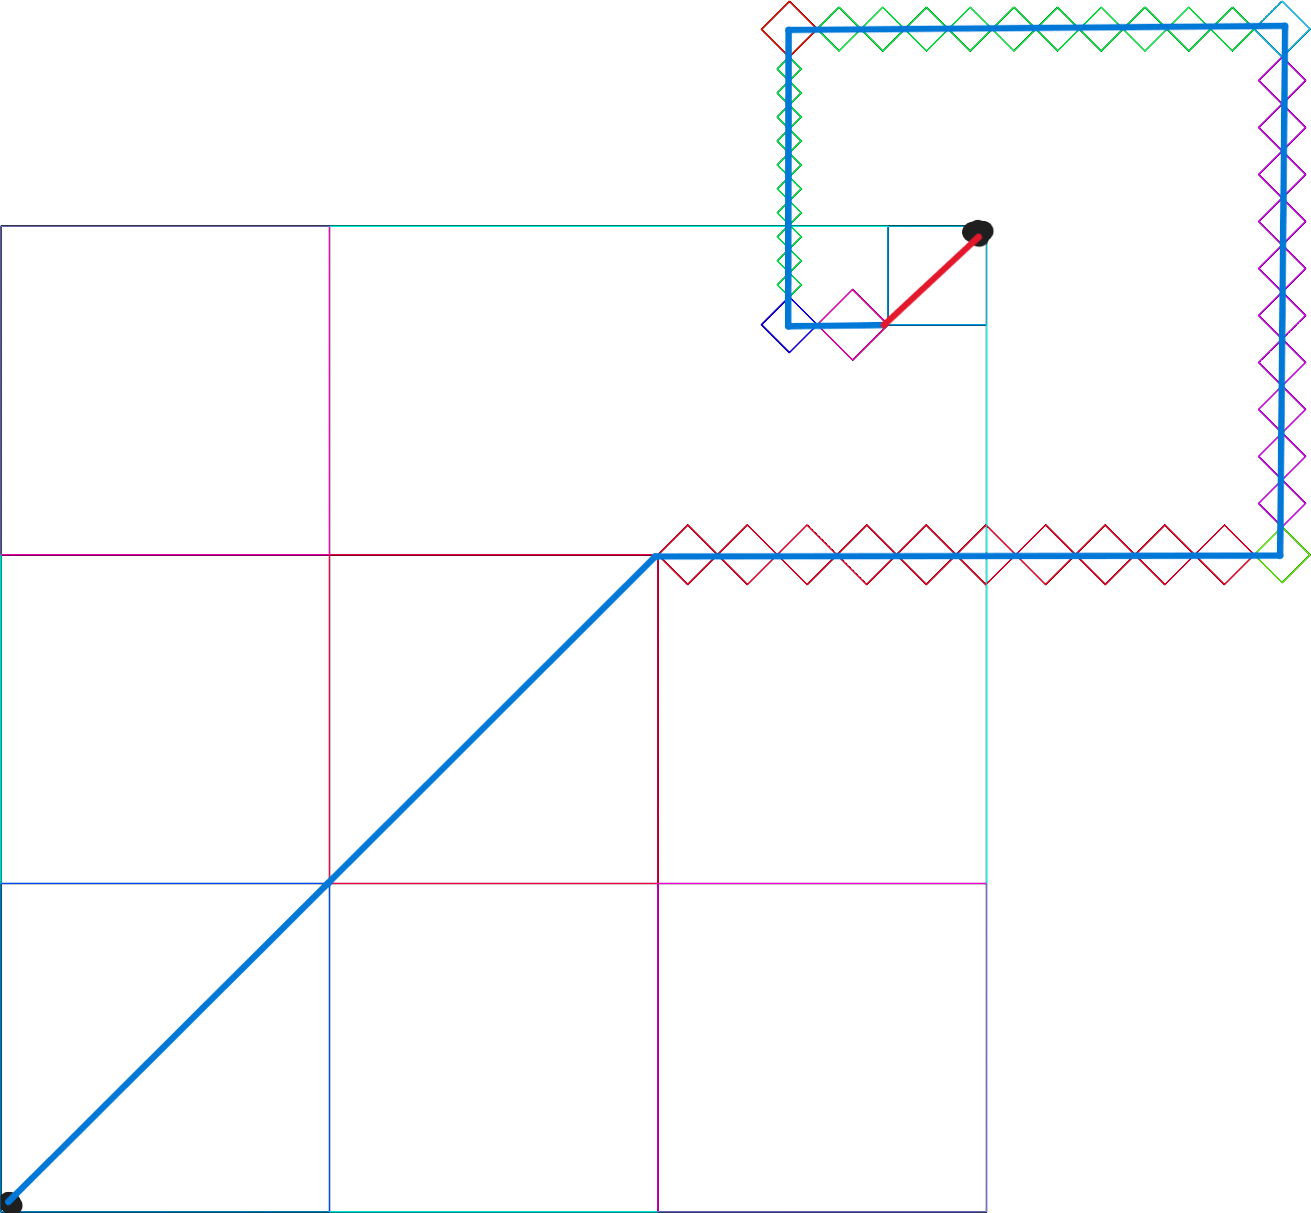
\includegraphics[width=0.45\textwidth]{superden2pi_P.png}
%\hfill
%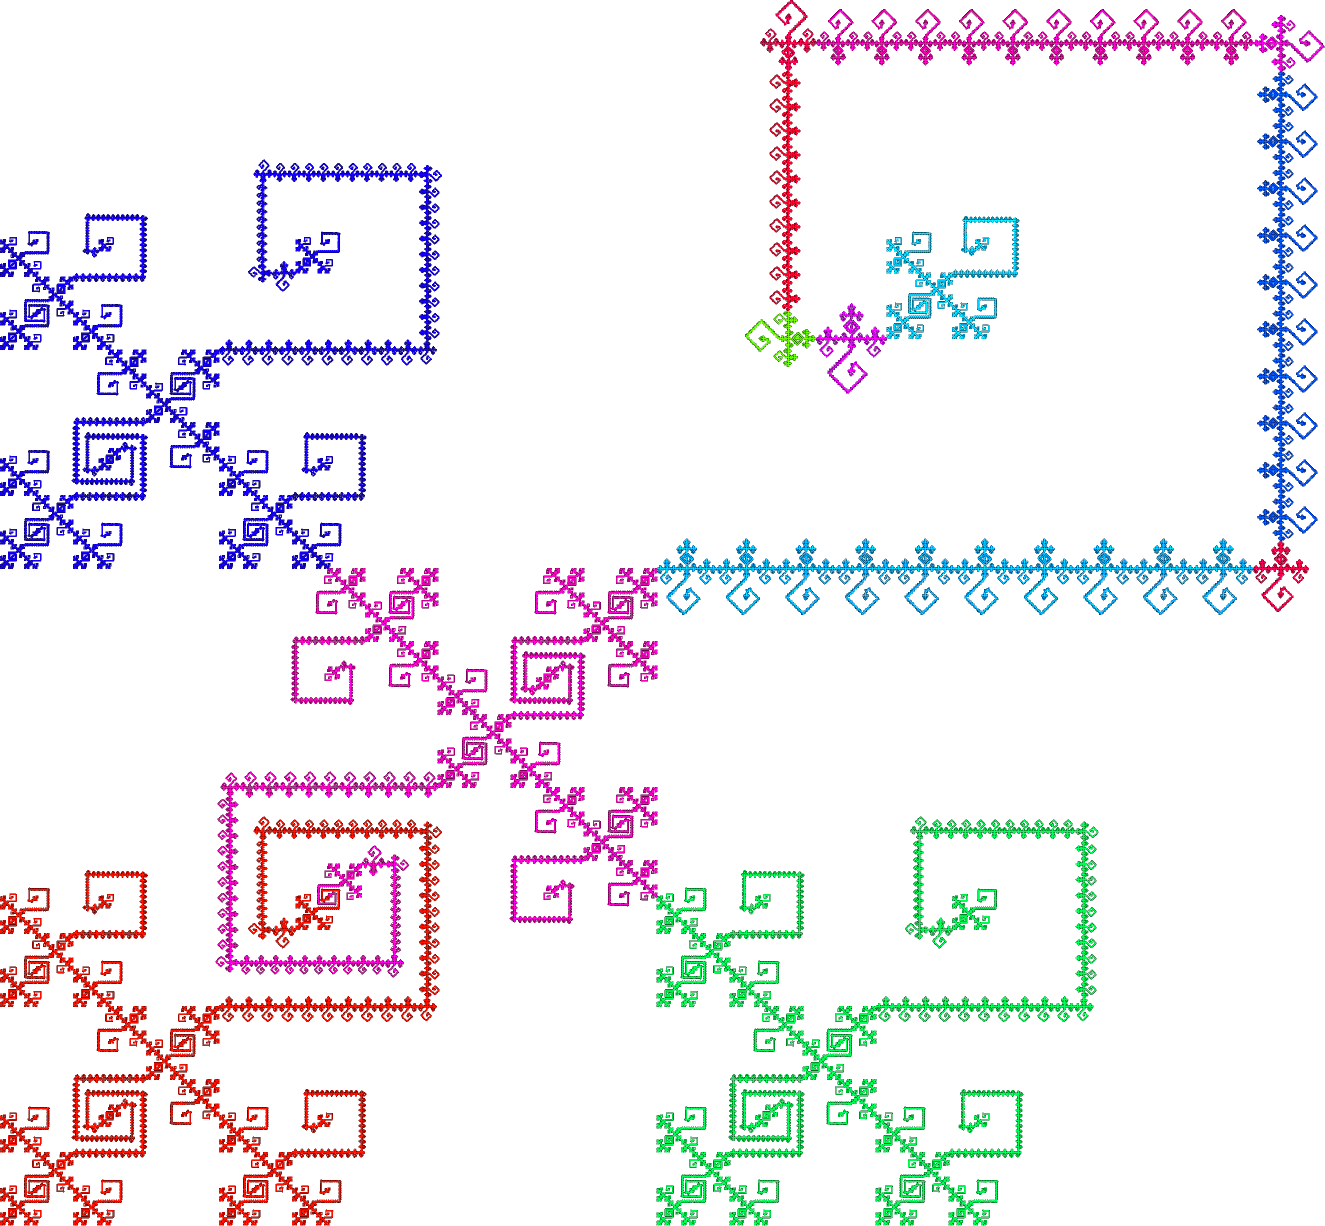
\includegraphics[width=0.45\textwidth]{superden2pi_K.png}
%\end{frame}


\begin{frame}{Полигональные системы и их деформации}{Основной результат: Теорема о совпадении параметров}
\begin{block}{Условие совпадения параметров}
% Для любых $B \in\cup_{i=1}^m  V_{P_i}$ и $A,A'$ таких, что, $S_i(A)=S_j(A')=B$, выполняется равенство $\lambda _i=\lambda _j$.
Обобщённая полигональная система система $\eS$ удовлетворяет условию совпадения параметров, если для каждого $x=S_i(P)\cap S_j(P)$ (при $i\neq j$) все инвариантные дуги $\gamma_i\IN S_i(K)$ и $\gamma_j\IN S_j(K)$) с концом в $x$ имеют относительно $x$ одинаковые параметры.
\end{block}
\begin{theorem}[Drozdov D., Samuel M., Tetenov A. (2021)]
Пусть аттрактор $K$ обобщенной полигональной системы $\eS$ является дендритом. 
Тогда система $\eS$ удовлетворяет условию совпадения параметров.
\end{theorem}
\end{frame}


\begin{frame}{Полигональные системы и их деформации}{Основной результат: Теорема о малых деформациях}
\begin{theorem}[Drozdov D., Samuel M., Tetenov A. (2021)]
Для каждой полигональной системы $\eS$ существует такое $\delta > 0$, что для всякой её $\delta$-деформации $\eS'$, удовлетворяющей условию совпадения параметров, аттрактор $K(\eS')$ является дендритом, изоморфным аттрактору $K(\eS)$.
\end{theorem}
% 1)$\da<\dfrac{q_{min}}{8};$  
% 2)$\da<\dfrac{(1-q_{max})}{8};$ 
% 3)$\da<\dfrac{\rho_0}{2(C_k+1)};$ 
% 4)$\da<\dfrac{\rho_1}{4(C_k+1)};$ 
% 5)$\da<\dfrac{1-\rho_2}{2(C_k+1)};$ 
% 6)$\da<\dfrac{\al_0}{\dfrac{2.1(C_k+1)}{\rho_1}+C_{\la}\log (\dfrac{1+3\rho_2}{3\rho_1})},$\\
% где $C_\al=2.1(1+1/q_{min}), C_K=\dfrac{28+4C_\al}{1-q_{max}}$, а $C_\la=\dfrac{2.1(1+1/q_{max})}{\log(3+q_{max})-\log(3q_{max}+1)}.$ 
\end{frame}



\section{Фрактальные $k$-кубы, являющиеся дендритами}


\begin{frame}{Фрактальные $k$-кубы, являющиеся дендритами}{История вопроса}
\begin{itemize}
    \item T. Bedford (1984); C. McMullen (1984) --- самоаффинные ковры Бедфорда-МакМаллена;
    \item Y. Peres (1994) --- условия, при которых мера ковров Бедфорда-МакМаллена несчётно-бесконечна;
    \item R. Kenyon, Y. Peres (1996) --- размерность и мера губок Серпинского;
    \item K. Lau, J.J. Luo, H. Rao (2013) --- топологические свойства замощений плоскости фрактальными квадратами;
    \item L. L. Cristea, B. Steinsky (2009, 2011, 2017, 2020) --- дуги во фрактальных квадратах и треугольниках;
    \item J. M. Fraser (2021) --- обзор по фрактальнм размерностям губок Серпинского;
\end{itemize}
\end{frame}


\begin{frame}{Фрактальные $k$-кубы, являющиеся дендритами}{Фрактальные $k$-кубы}

\begin{definition}
Пусть  $D=\{d_1,\ldots,d_r\},\; d_i\in\{0,1,\ldots,n-1\}^k$, где $n\ge 2$, а $1<\#D<n^k$.\\
{\em Фрактальным $k$-кубом порядка $n$ с множеством единиц $D$} называют компактное множество $K\IN\rr^k$, удовлетворяющее равенству\\
\center{$K=\dfrac{K+D}{n}.$}
\end{definition}

\qquad\qquad
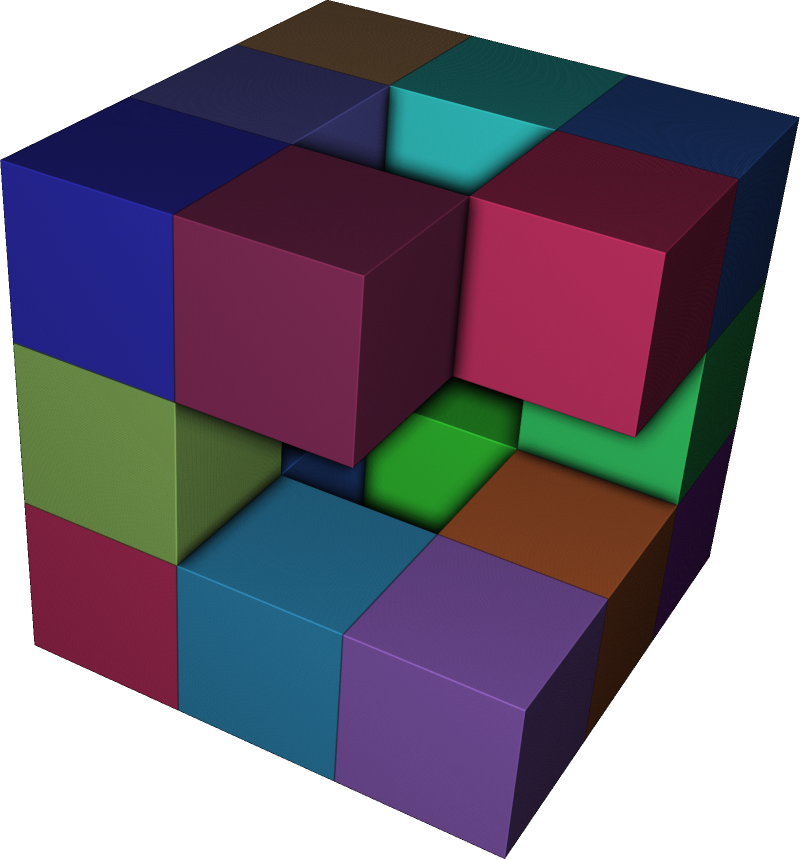
\includegraphics[width=0.3\textwidth]{FQD.png}
\hfill
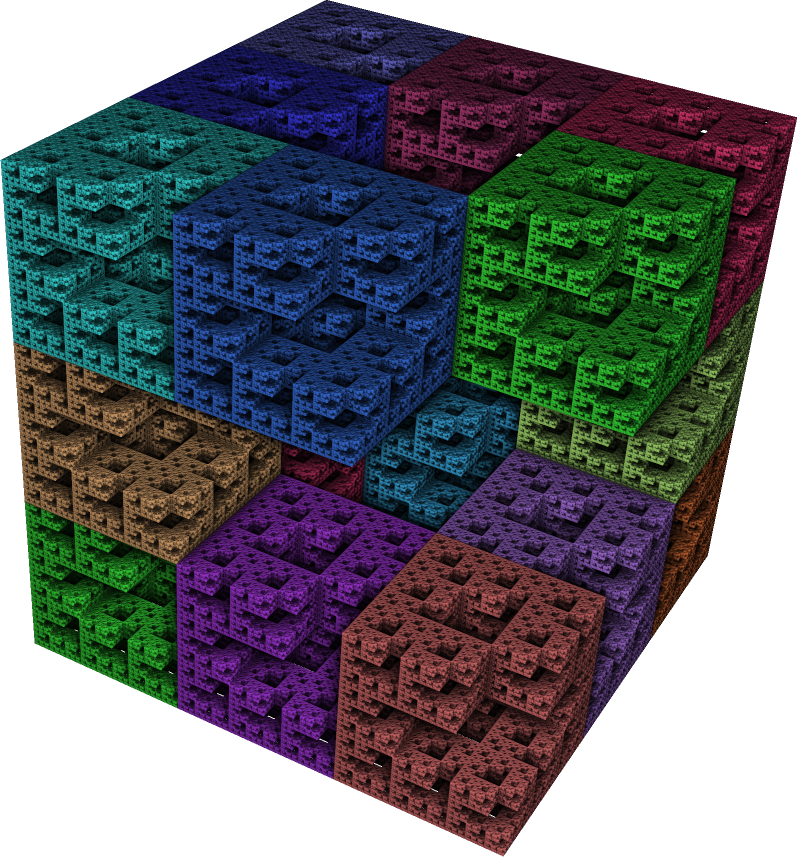
\includegraphics[width=0.3\textwidth]{FQK.png}
\qquad\qquad
\end{frame}


\begin{frame}{Фрактальные $k$-кубы, являющиеся дендритами}{Основной результат:Теорема о пересечениях граней фрактальных $k$-кубов }
Пусть в дальнейшем $K^1$ и $K^2$ --- фрактальные $k$-кубы порядка $n$ с множествами единиц $D^1$ и $D^2$.
Для любого $\bma\in A$ символом $F_\bma=K^1_\bma\cap(K^2_{-\bma}+\bma)$.
%Уравнения, задающие множества $F_\bma$, получаются из следующей теоремы.

\begin{theorem}\label{IFC}
Семейство множеств $\{F_\bma=K^1\cap(K^2+\bma)\ :\ \bma\in A\}$ удовлетворяет системе $\Sa$ уравнений 
$$F_\bma=\bigcup\limits_{\bmb\sqsupseteq\bma} 
\dfrac{F_\bmb+G_{\bma\bmb}}{n},$$
где $G_{\bma\bmb}=D^1\cap(D^2+n\bma-\bmb)$.
\end{theorem}
Множество $G_{\bma\bma}=D^1\cap(D^2+(n-1)\bma)$ мы обозначим как $G_{\bma}$.
\end{frame}


%\begin{frame}{Структурный граф}
%\only<1>{
%\begin{lemma}
%Множество $F_\bma=\0$ тогда и только тогда, когда для любого $\bmb\sqsupseteq\bma$ и для любой цепочки $\bma=\bma_0\sqsubseteq\bma_1\sqsubseteq\ldots \bma_{p-1}\sqsubseteq\bma_p=\bmb$ произведение 
%$\#G_{\bma_0\bma_1}\cdot\#G_{\bma_1\bma_2}\cdot\ldots\cdot\#G_{\bma_{p-1}\bma_p}\cdot\#G_{\bmb}$ равно нулю. 
%\qed
%\end{lemma} 
%
%Отношения между множествами $F_\bma$ описываются {\em структурным графом $\Ga_\Sa$} системы $\Sa$. 
%
%\begin{definition}
%Структурным графом $\Ga_\Sa$ называется отмеченный ориентированный граф с множеством вершин $\{\bma\in A\ :\ F_\bma\neq\0\}$ и множеством рёбер $\{(\bma, \bmb)\ :\ \bma\sqsubseteq\bmb, G_{\bma\bmb}\neq\0, F_\bmb\neq\0\}$, где ребро $(\bma, \bmb)$ направлено из $\bma$ в $\bmb$ и отмечено $G_{\bma\bmb}$.
%\end{definition}}
%\only<2>{
%\center{
%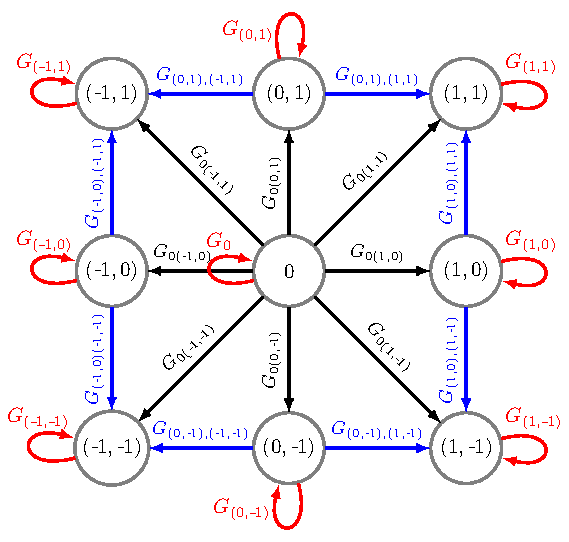
\includegraphics[width=.6\textwidth]{structure_graph_full_new.pdf}}
%}
%\end{frame}




\begin{frame}{Фрактальные $k$-кубы, являющиеся дендритами}{Основной результат: Мощность множества $F_\bma$}
\begin{theorem}
\begin{itemize} %[nolistsep]
\item[(1)] Если $\#G_\bmb>1$ для некоторого $\bmb\succcurlyeq\bma$, то  $F_\bma$ несчётно.

\item[(2a)] Если  $\#G_\bmb\leq1$ для любого $\bmb\succcurlyeq\bma$, то  $F_\bma$ не более чем счетно.

\item[(2b)] Если при этом существует $\bmb'\succ\bmb$ такое, что $\#G_\bmb=1$ и $F_{\bmb'}\neq\0$, то $F_\bma$ счетно.

\item[(3)] Если  $\#G_\bmb=1$ для всех максимальных вершин $\bmb$ в $\Gamma_\bma$, и $G_{\bma_i}=\0$ для всех остальных вершин $\bma_i$ в $\Gamma_\bma$, то $F_\bma$ конечно.
%В этом случае $\#F_\bma$ не превосходит сумму произведений $\prod \limits_{j=1}^{p-1}\# G_{\bma_j\bma_{j+1}}$, взятых по всем цепочкам $\bma=\bma_1\prec\ldots\prec\bma_p=\bmb$, где $\bmb$  максимальна в $\Gamma_\bma$.

\item[(4)] Если все $\bma_i\succcurlyeq\bma$ образуют единственную цепочку $\bma=\bma_1\prec\ldots\prec\bma_p$, в которой $G_{\bma_j}=\0$ и $\# G_{\bma_j\bma_{j+1}}=1$, $\#G_{\bma_p}=1$ для всех $j\le p-1$, то $\#F_\bma=1$.
\end{itemize}
\end{theorem}
\end{frame}



\begin{frame}{Фрактальные $k$-кубы, являющиеся дендритами}{Основной результат: Алгоритм проверки фрактального $k$-куба}

%Чтобы проверить, является ли фрактальный $k$-куб $K$ дендритом с одноточечным пересечением, нужно выполнить следующие шаги:

\begin{enumerate}

\item  Найдём все множества $G_\bma, G_{\bma\bmb}$ и выпишем систему уравнений $\Sigma$.
Если $F_0=\0$, то $K$ несвязен и не может быть дендритом.

\item  Построим для системы $\Sa$ её структурный граф $\Ga_\Sa$.
Если граф $\Ga_\Sa$ несвязен, то рассматриваем подграф $\Ga_0$.
 
\item  Проверим, является ли $K$ множеством с одноточечным пересечением.
Если это не так, то $K$ не является дендритом с одноточечным пересечением.
    
\item  Построим двудольный граф пересечений $\hat\Gamma$ для фрактального куба $K$.
При этом следует учесть случаи, когда чёрная вершина в $\hat\Gamma$ соединена более чем с двумя белыми вершинами.

\item  Если получившийся двудольный граф пересечений $\hat\Gamma$ является деревом, то $K$ --- дендрит с одноточечным пересечением.    
\end{enumerate}
\end{frame}


\section{Фрактальные квадраты с конечным пересечением}


\begin{frame}{Фрактальные квадраты с конечным пересечением}{Основной результат: Критерий дендритности фрактального квадрата}

Множество $F_\bma$ одноточечно, если \\
\textbf{(a)} $\#G_{\bma\bma}=1$ и $\#F_\bmb\cdot\#G_{\bma\bmb}=0$ для каждого $\bmb\sqsupset\bma$; или\\
\textbf{(b)} $\#G_{\bma\bma}=0$ и существует $\bmb\sqsupset\bma$ такое, что $\#F_\bmb\cdot\#G_{\bma\bmb}=1$.

\begin{proposition}
Если фрактальный квадрат $K$ является дендритом, то он обладает свойством одноточечного пересечения.
\end{proposition}
\begin{corollary}
Фрактальный квадрат $K$ является дендритом тогда и только тогда, когда его двудольный граф пересечений является деревом.
\end{corollary}
%\begin{center}
%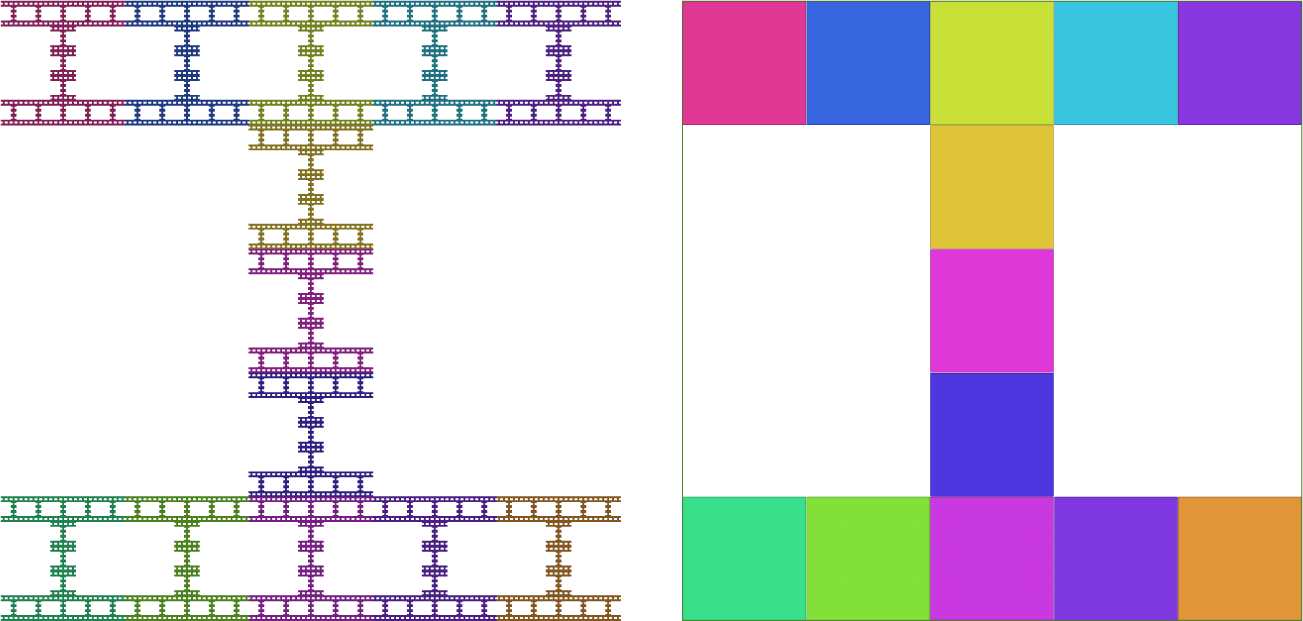
\includegraphics[width=0.8\textwidth]{line_int.png}
%\end{center}
\end{frame}


\begin{frame}{Фрактальные квадраты с конечным пересечением} {Самоподобная граница односвязных фрактальных квадратов}
\begin{theorem}\label{ssboundary}
Пусть $K$ --- фрактальный квадрат, являющийся дендритом и не являющийся отрезком.
Тогда $\#\dd K\in\{3,\ 4,\ 6\}$. \\
Если $\#\dd K=4$, то  $\dd K=F_\bma\cup F_{-\bma}\cup F_\bmb\cup F_{-\bmb}$, где   пара  $\bma,\bmb$ принимает одно из следующих значений:
	\begin{itemize}%[nolistsep]
	\item[{\bf A.}] $\bma=(1,0)$, $ \bmb=(0,1)$;
	\item[{\bf B.}] $\bma=(1,1)$, $ \bmb=(1,-1)$;
	\item[{\bf C.}] $\bma\in\{(1,1),\ (1,-1)\},\bmb\in\{(1,0),\ (0,1)\}$.
	\end{itemize}
 Если $\#\dd K=3$ или $\#\dd K=6$, то
\begin{itemize}%[nolistsep]
	\item[{\bf D.}] $\dd K=F_{(1,0)}\cup F_{(-1,0)}\cup F_{(0,1)}\cup F_{(0,-1)}\cup F_\bmb\cup F_{-\bmb}$, где $\bmb\in\{(1,1),\ (1,-1)\}$.
	\end{itemize}
\end{theorem}
\end{frame}


%\begin{frame}{
%\only<1>{Типы \textbf{A}, \textbf{B} и \textbf{C}}
%\only<2>{Типы \textbf{D3} и \textbf{D6}}}
%\begin{center}
%\only<1>{
%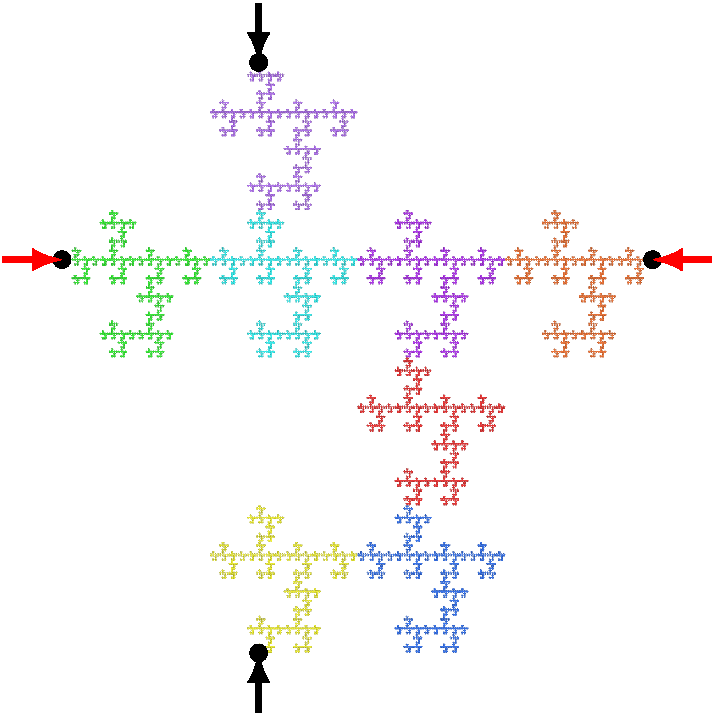
\includegraphics[width=0.3\textwidth]{A_type.pdf}
%\hfill
%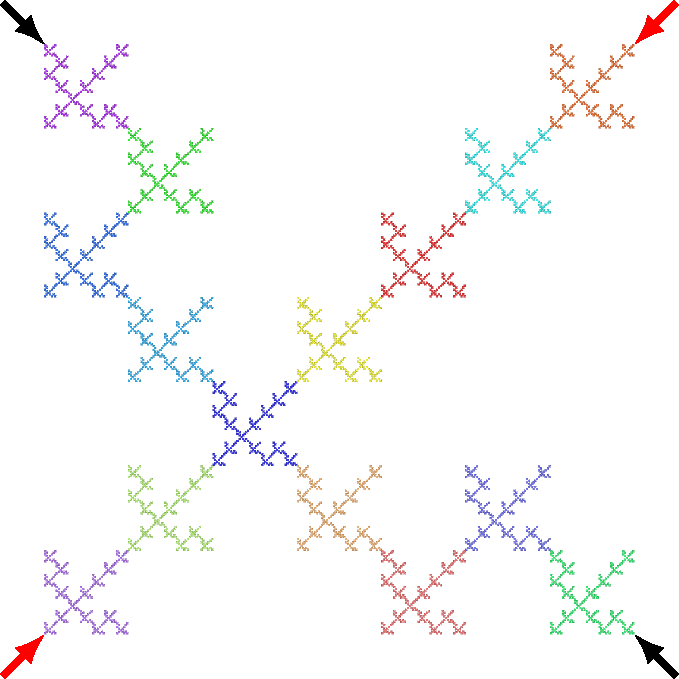
\includegraphics[width=0.3\textwidth]{B_type.pdf}
%\hfill
%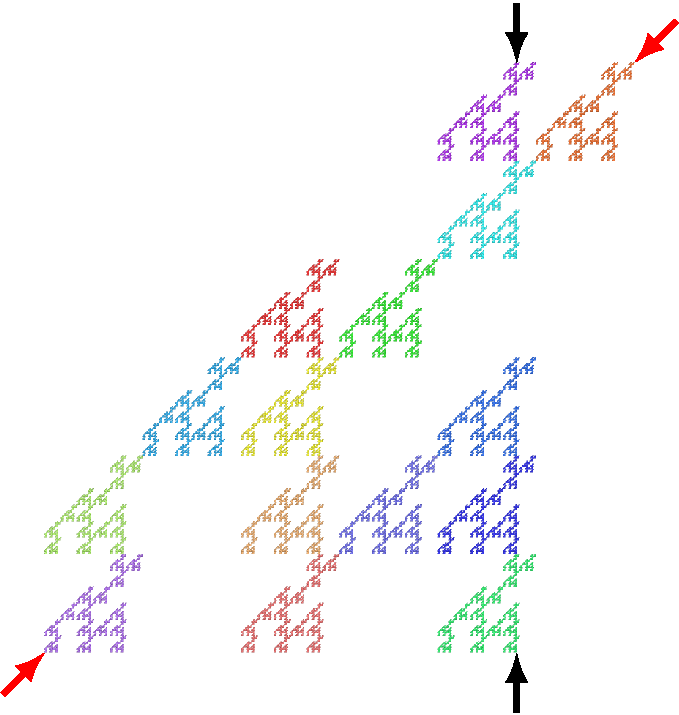
\includegraphics[width=0.3\textwidth]{C_type.pdf}}
%\only<2>{
%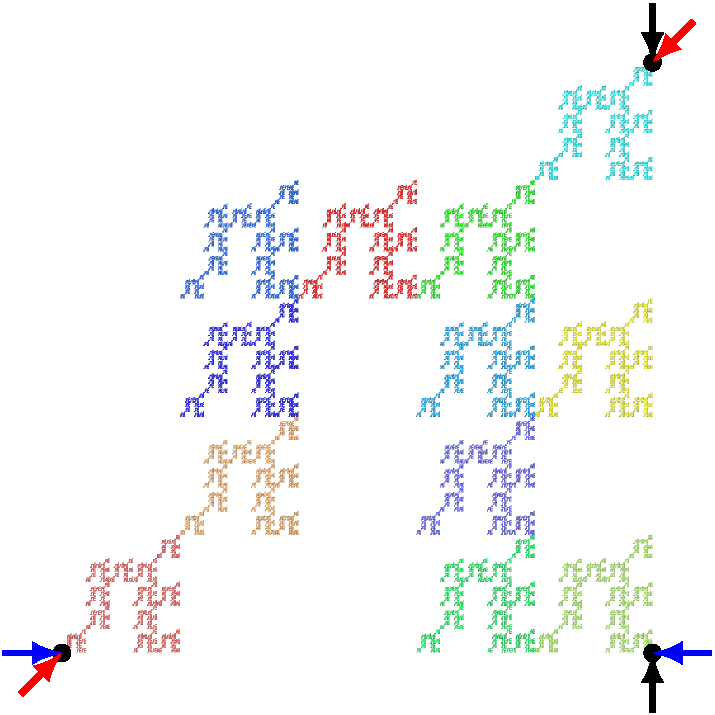
\includegraphics[width=0.4\textwidth]{D3_type.pdf}
%\hfill
%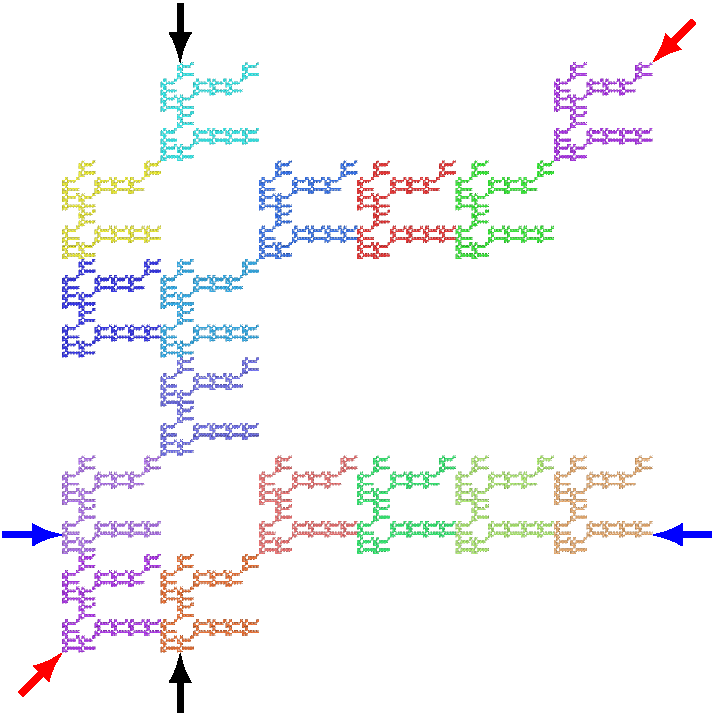
\includegraphics[width=0.4\textwidth]{D6_type.pdf}}
%\end{center}
%\end{frame}


\begin{frame}{Фрактальные квадраты с конечным пересечением}{Основной результат: Классификация фрактальных квадратов}

\begin{theorem}[Tetenov A., Drozdov D.  (2023)]
Для фрактальных квадратов, являющихся дендритами, существует только $7$ типов главного дерева, модели которых показаны ниже.
\end{theorem}

\includegraphics{mt1.pdf}
\hfill
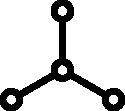
\includegraphics{mt2.pdf}
\hfill
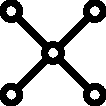
\includegraphics{mt3.pdf}
\hfill
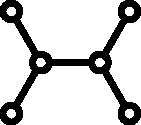
\includegraphics[width=2.2cm]{mt4.pdf}\\
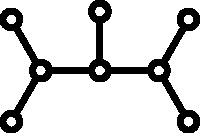
\includegraphics[width=2.5cm]{mt5.pdf}
\hfill
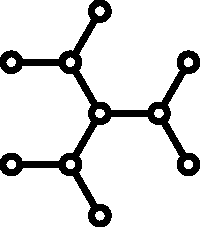
\includegraphics[width=2.3cm]{mt6.pdf}
\hfill
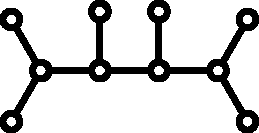
\includegraphics[width=3.2cm]{mt7.pdf}
\end{frame}

\section{Апробация результатов}
\begin{frame}{Апробация результатов}

{\normalsize
\begin{thebibliography}{9}
{\small
\bibitem{DST2021}
{\bf Drozdov D., Samuel M., Tetenov A.},
On deformation of polygonal dendrites preserving the intersection graph //
The Art of Discrete and Applied Mathematics. 2021. Т. 4. № 2. С. 1--21.

\bibitem{DST2022}
{\bf Drozdov D., Samuel M., Tetenov A.}, 
On $\delta$-deformations of Polygonal Dendrites // 
Topological Dynamics and Topological Data Analysis. : Springer Singapore, 2021. С. 147--164.

\bibitem{DT2024fqd}
{\bf Drozdov D. A., Tetenov A. V.}, On the dendrite property of fractal cubes // Advances in the Theory of Nonlinear Analysis and Its Application. 2024. Т. 8. № 1. С. 73--80.

\bibitem{TD2022fs}
{\bf Drozdov D., Tetenov A.}, 
On fractal squares possessing finite intersection property // 
Bulletin of National University of Uzbekistan: Mathematics and Natural Sciences. 2022. Т. 5. № 3. С. 164--181.

\bibitem{TD2023fs}
{\bf Drozdov D., Tetenov A.}, 
On the classification of fractal square dendrites // 
Advances in the Theory of Nonlinear Analysis and Its Application. 2023. Т. 7. № 3. С. 19--96.

\bibitem{VDT2020}{\bf Ваулин Д. А., Дроздов Д. А., Тетенов А. В.},
О связных компонентах фрактальных кубов // 
Труды Института математики и механики УрО РАН. 2020. Т. 26. № 2. С. 98--107.}
\end{thebibliography}}
\end{frame}

\section{}
\begin{frame}{}
\begin{center}
\Huge Благодарю за внимание
\end{center}
\end{frame}


\end{document}